\chapter{Methodology}
\label{chap:2}
\ChapterPageStuff{2}

\section{Preamble}
In this chapter the methodology to create and implement a logging mechanism to do system utilisation analysis on software system will be discussed. \Cref{sec:EventLogging} provided the necessary literature to create a logging mechanism in \Cref{sec:Ch3_LoggingMechanism} for two software systems.

\section{Logging mechanism}\label{sec:Ch3_LoggingMechanism}
For this study two software systems are used to implement two different logging mechanisms. The first software system which will be called System A, is energy management system that uses \emph{PHP}. System B is a \emph{.NET Framework}\footnote{\label{ftn:NetFramework}\textbf{.NET Framework} is a run-time execution environment that consists of common language run-time (\emph{CLR}) and a \texttt{.NET Framework Class Library} \cite{Harkness2007}.} system with a \emph{MVC} architecture as in \Cref{fig:ch2_Flow_MVC_Architecture} and is the administrative software system to configure System A.

\subsection{System A}
Logging point are essential data that describes the event's key features when creating a log as discussed in \Cref{sec:Ch1_LoggignPoints}. Both System A and B have certain key logging points that needs to be obtained from the user generated event.

\subsubsection{System A's logging points}\label{sec:SystemA_LoggingPoints}
In \Cref{fig:ch2_SystemA_Dashboard} each mine group have multiple toolboxes linked to them. They can be same toolbox linked to both mine groups such as \emph{T1} and \emph{T3}. These toolboxes represent a group of dashboards related to the aspects of energy management of mines.\par Each of these toolboxes have a dashboards linked to them and each mine group can have different dashboards linked to the to the same toolbox. Each one of these mine groups, toolboxes and dashboards forms part of System A's web pages which the user can access where event logs are generated.

\begin{figure}[!htb] % An h :here, t: top, b: bottom.
	\centering % cent the figure
	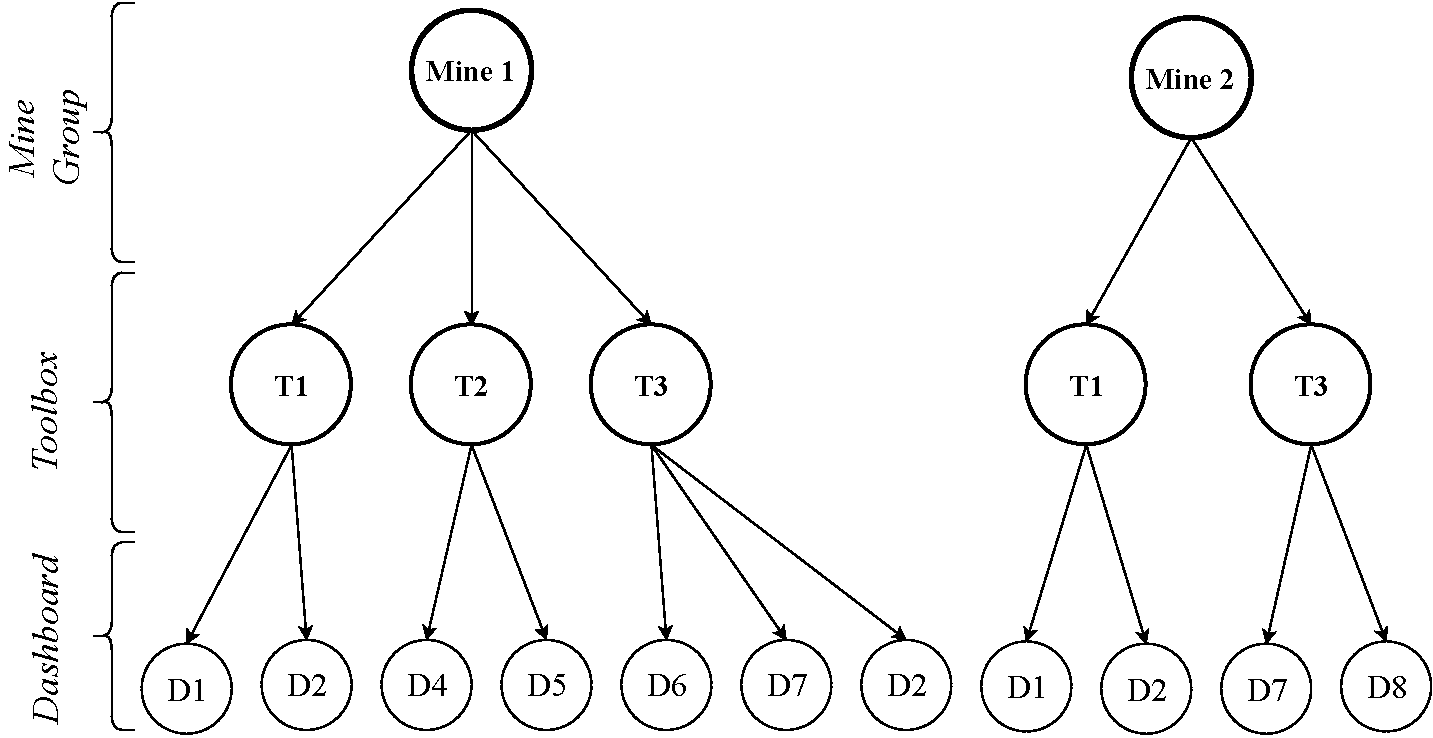
\includegraphics[width=0.8\textwidth]{Chapter2/SystemA_Dashboard/SystemA_Dashboard.pdf}
	\caption[System A dashboard links]
	{\textit{System A dashboard links}}\label{fig:ch2_SystemA_Dashboard}
\end{figure}

Each dashboard in \Cref{fig:ch2_SystemA_Dashboard} can use the same files to create the a dashboard by only configuring the content of the dashboard based on the request parameters that is send when the user navigates to a new dashboard. Capturing the user generated events with a logging mechanism can be done in these shared files instead of the entire software components of System A.\par The user session helps to keep to track of any information needed for these pages to be fully functional like the user's identity and dashboard related data. This information can be used to give insight on which page the user is currently active on. In this case for System A the important user session information is:

\begin{itemize}
	\item \textbf{User's identity:} The session contains the user's name and identity number which is the unique primary key for the user. This session information will always be available if the user is active on the software system from the instance they are logged in and verified until the user logs out and close their browser.
	\item \textbf{Group identity:} System A is used for multiple mine companies, each of the mining companies have a unique identity number. Each group have multiple toolboxes linked to them for energy management.
	\item \textbf{Dashboard identity:} Each dashboard uses certain files to construct a web page the user can view. To correctly navigate and get the correct page when the user request it, a unique identity number is used. In some cases for this system the same file can be used for multiple dashboards as extra configuration data is obtained from the database for that specific dashboard identity number.
	\item \textbf{Configuration meta data identity:} In \Cref{fig:ch2_SystemA_Dashboard} the same dashboard can be linked to different mine groups or toolboxes. The user session contains any other identification parameters of which meta data should be loaded to configure the dashboard for the correct mine group and toolbox.
\end{itemize}

\begin{table}[!htb]
	\centering
	\small
	\caption[System A user activities logging points]
	{\textit{System A user activities logging points}}
	\label{tbl:Ch2_System_A_Logging_Points}
	\begin{tabularx}{\textwidth}{|l|l|X|}
		\hline \textbf{Column Name} & \textbf{SQL Data Type} & \textbf{Description} \\
		\hline \textbf{ActivityID} & INT(11) & The activity identification is an incremental number of the event that is logged.\\
		\hline \textbf{Timestamp} & DATETIME & This is the time which the event took place.\\
		\hline \textbf{UserID} & INT(45) & Each user has a unique identifier which is a numerical identification number that is foreign key reference to the User table.\\
		\hline \textbf{DashboardID} & INT(4) & Foreign key reference to the Dashboard table. \\
		\hline \textbf{GroupID} & INT(4) & This foreign key reference to the Group table is contract groups identification number. \\ 		
		\hline \textbf{ActivityType} & ENUM & Each event that user initiated has an activity type as in \Cref{tbl:Ch2_SystemA_EventTypes}. \\
		\hline \textbf{File} & VARCHAR(200) & This the PHP file from which the request is processed.\\
		\hline \textbf{RequestParameters} & JSON & Request parameters of the event. This can be other meta data that is important about the user's activity using certain controls on a dashboard or toolbox. \\
		\hline
	\end{tabularx}
\end{table}

\clearpage

Obtaining the key information of the user generated event is essential to define which key logging points the logging mechanism needs to get from the user's session. In \Cref{tbl:Ch2_System_A_Logging_Points} System A's key logging points which are saved in a SQL database. Each logging point can be accessed either by the user session or other run-time data present when the event took place such as any meta data that as send back the server as request parameters.

The user activity types in \Cref{tbl:Ch2_SystemA_EventTypes} is all of the possible activities the user can generate in System A. The DetailView activities is expected to the largest portion of events that will be tracked as users will generally try to use multiple input elements on the dashboard or toolbox. \par The Dash event type is only useful to track which dashboards and toolboxes the user navigates to and it will not be accurate indicator to how much a dashboard or toolbox is used. The DetailView and Report user activity types is better representation of the utilisation of these software components as these events are the user's objectives using the software systems and not trying access the software systems.  

\begin{table}[!htb]
	\centering
	\small
	\caption[System A user activity types]
	{\textit{System A user activity types}}
	\label{tbl:Ch2_SystemA_EventTypes}
	\begin{tabularx}{\textwidth}{|l|X|}
		\hline \textbf{Activity Type} & \textbf{Description} \\
		\hline \textbf{Dash} & Any activity that the user attempts to access a toolbox or dashboard on System A is Dash event type. \\
		\hline \textbf{DetailView} & Any other activities such as viewing certain date's data or editing and saving activities on System A is DetailView events and have other meta data which is the request parameters send back to server. These events exclude Report events. \\
		\hline \textbf{Report} & There are multiple detailed reports generated on these dashboards which are classified as Report events. \\
		\hline
	\end{tabularx}
\end{table}

Using the key logging points of \Cref{tbl:Ch2_System_A_Logging_Points} the \emph{ERD} for all the tables used to for System A user activity logging data is created in \Cref{fig:Ch2_SystemA_Basic_ERD}. Table SystemA\_UserActvities is where all the user activity tracking data is stored in a SQL database with foreign key references to the Dashboards, Users and Groups tables.

\begin{figure}[!htb] % An h :here, t: top, b: bottom.
	\centering % cent the figure
	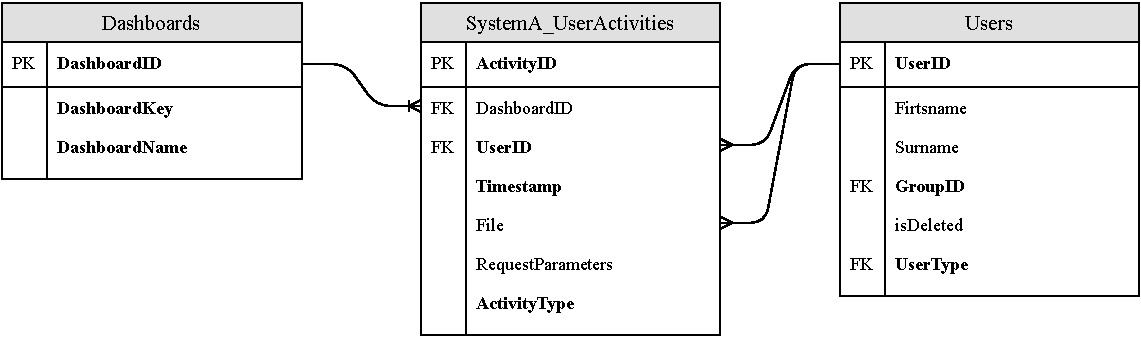
\includegraphics[width=0.9\textwidth]{Chapter2/SystemA_ERD_Basic/SystemA_ERD_Basic.pdf}
	\caption[System A user activity ERD]
	{\textit{System A user activity ERD}}\label{fig:Ch2_SystemA_Basic_ERD}
\end{figure}

\clearpage

In \Cref{fig:CH2_SystemBMetaData} is the meta data JSON for the RequestParameters column in \Cref{tbl:Ch2_System_A_Logging_Points}. This JSON contains certain data parameters important to the event that the user has initiated. This request parameters will need to be specified for each toolbox and dashboard the user events are logged of for System A.

\begin{figure}[!htb]
	\centering
	\begin{lstlisting}[style=json] 
	{
		"Parameter1": 4,
		"Parameter2": "Hello World!",
		"Parameter3": true
		"Parameter4": 40.404
	}
	\end{lstlisting}
	\caption[System A meta data JSON]
	{\textit{System A meta data JSON}}\label{fig:CH2_SystemAMetaData}
\end{figure}

\subsubsection{System A logging mechanism design}
\Cref{sec:SystemA_LoggingPoints} the logging points System A's key logging points need to be captured by a logging mechanism. In \Cref{fig:ch2_SystemA_Arch_Design} is the design for the System A's logging mechanism to effectively log the user generated event from the PHP software components. The logging mechanism consist of two main functional requirements (\textbf{F/R}) which is the client and server functional requirements.

\begin{figure}[!htb] % An h :here, t: top, b: bottom.
	\centering % cent the figure
	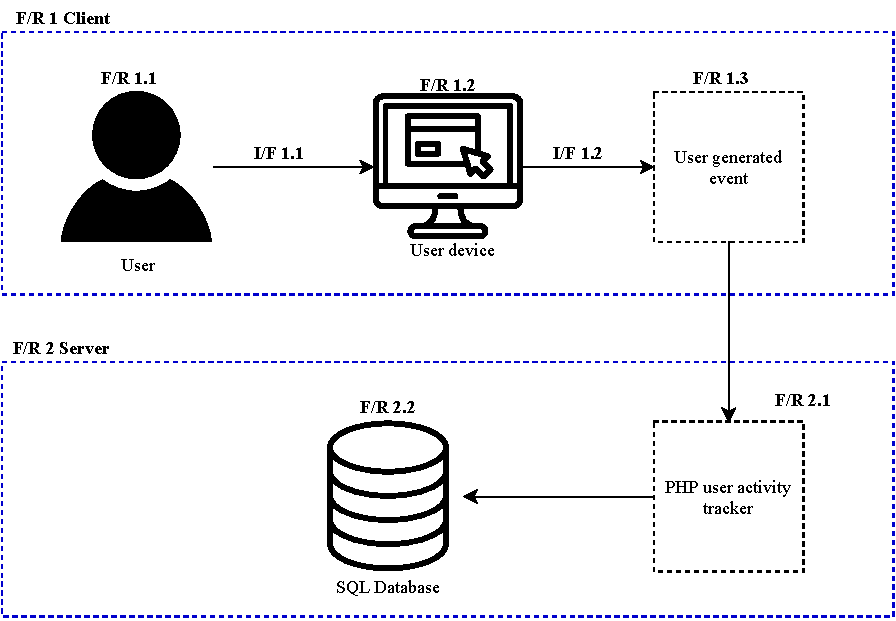
\includegraphics[width=0.9\textwidth]{Chapter2/SystemA_Architecture_Diagram/SystemA_Architecture_Diagram.pdf}
	\caption[System A logging mechanism architecture design]
	{\textit{System A logging mechanism architecture design}}\label{fig:ch2_SystemA_Arch_Design}
\end{figure}

In the client's functional requirements (F/R 1) the user the is main focus and is the initiator of user activity event logs that take place in System A. The user has a direct interface (I/F 1.1) to the device (F/R 1.2) that is currently browsing System A's websites for specific tasks.\par If the user initiates an activity the request will in most cases either be handled in the dashboard manager of System A or on a defined file where the dashboards software components are. These activities are either captured by the logging mechanisms of \Cref{fig:ch2_Dash_PHP_Flow} or \Cref{fig:ch2_DetailView_Flow} that gets the necessary parameters and defines the type of the user generated event of \Cref{tbl:Ch2_SystemA_EventTypes}. \par The user generated event (F/R 1.3) is send to the user activity tracker logger (F/R 2.1) which is the database interaction of the logging mechanism as in \Cref{fig:CH2_SystemA_DB_Interaction_FlowDiagram} to create a log entry in the SQL database of (F/R 2.2).

\subsubsection{Dash user activty type classification}

In \Cref{fig:ch2_Dash_PHP_Flow} is the process of getting the Dash and Report user activity event type for System A. In System A there are certain software components in a dashboard manager file that manages the dashboards according to which the user has selected to view. This dashboard manager file will always be execute the needed processes to manage the dashboard upon is start-up phase.\par When the user sends a request a to view a dashboard the requested dashboard's ID send to the dashboard manager. The dashboard manager will attempt to get the dashboard based on the provided dashboard ID. If the request doesn't contain a dashboard ID parameter, any attempt to log the activity will be ended and will be handled with the logging process described in \Cref{fig:ch2_DetailView_Flow}. \par If the dashboard ID parameter does exist and is not an empty or null value it will be added to the activity parameters. The activity parameters consist of some of the parameters needed for \Cref{tbl:Ch2_System_A_Logging_Points} when the event log is eventually saved in the database. \par In System A there are reports generated and some of the events of the report generation will use the dashboard manager's file. These user generated events can only be traced there and will send an action parameter that is use to initiate the report generation process.\par The action parameters in System A is parameters set in the Post and Get methods. If the action parameter contains report generation value the activity type needs to be set to the Report user activity type otherwise it is set the Dash user activity type. After the additional parameters and activity type parameters are set the ActivityTracker function is called to complete the log and save it in the SQL database as in \Cref{fig:CH2_SystemA_DB_Interaction_FlowDiagram}. 

\begin{figure}[!htb] % An h :here, t: top, b: bottom.
	\centering % cent the figure
	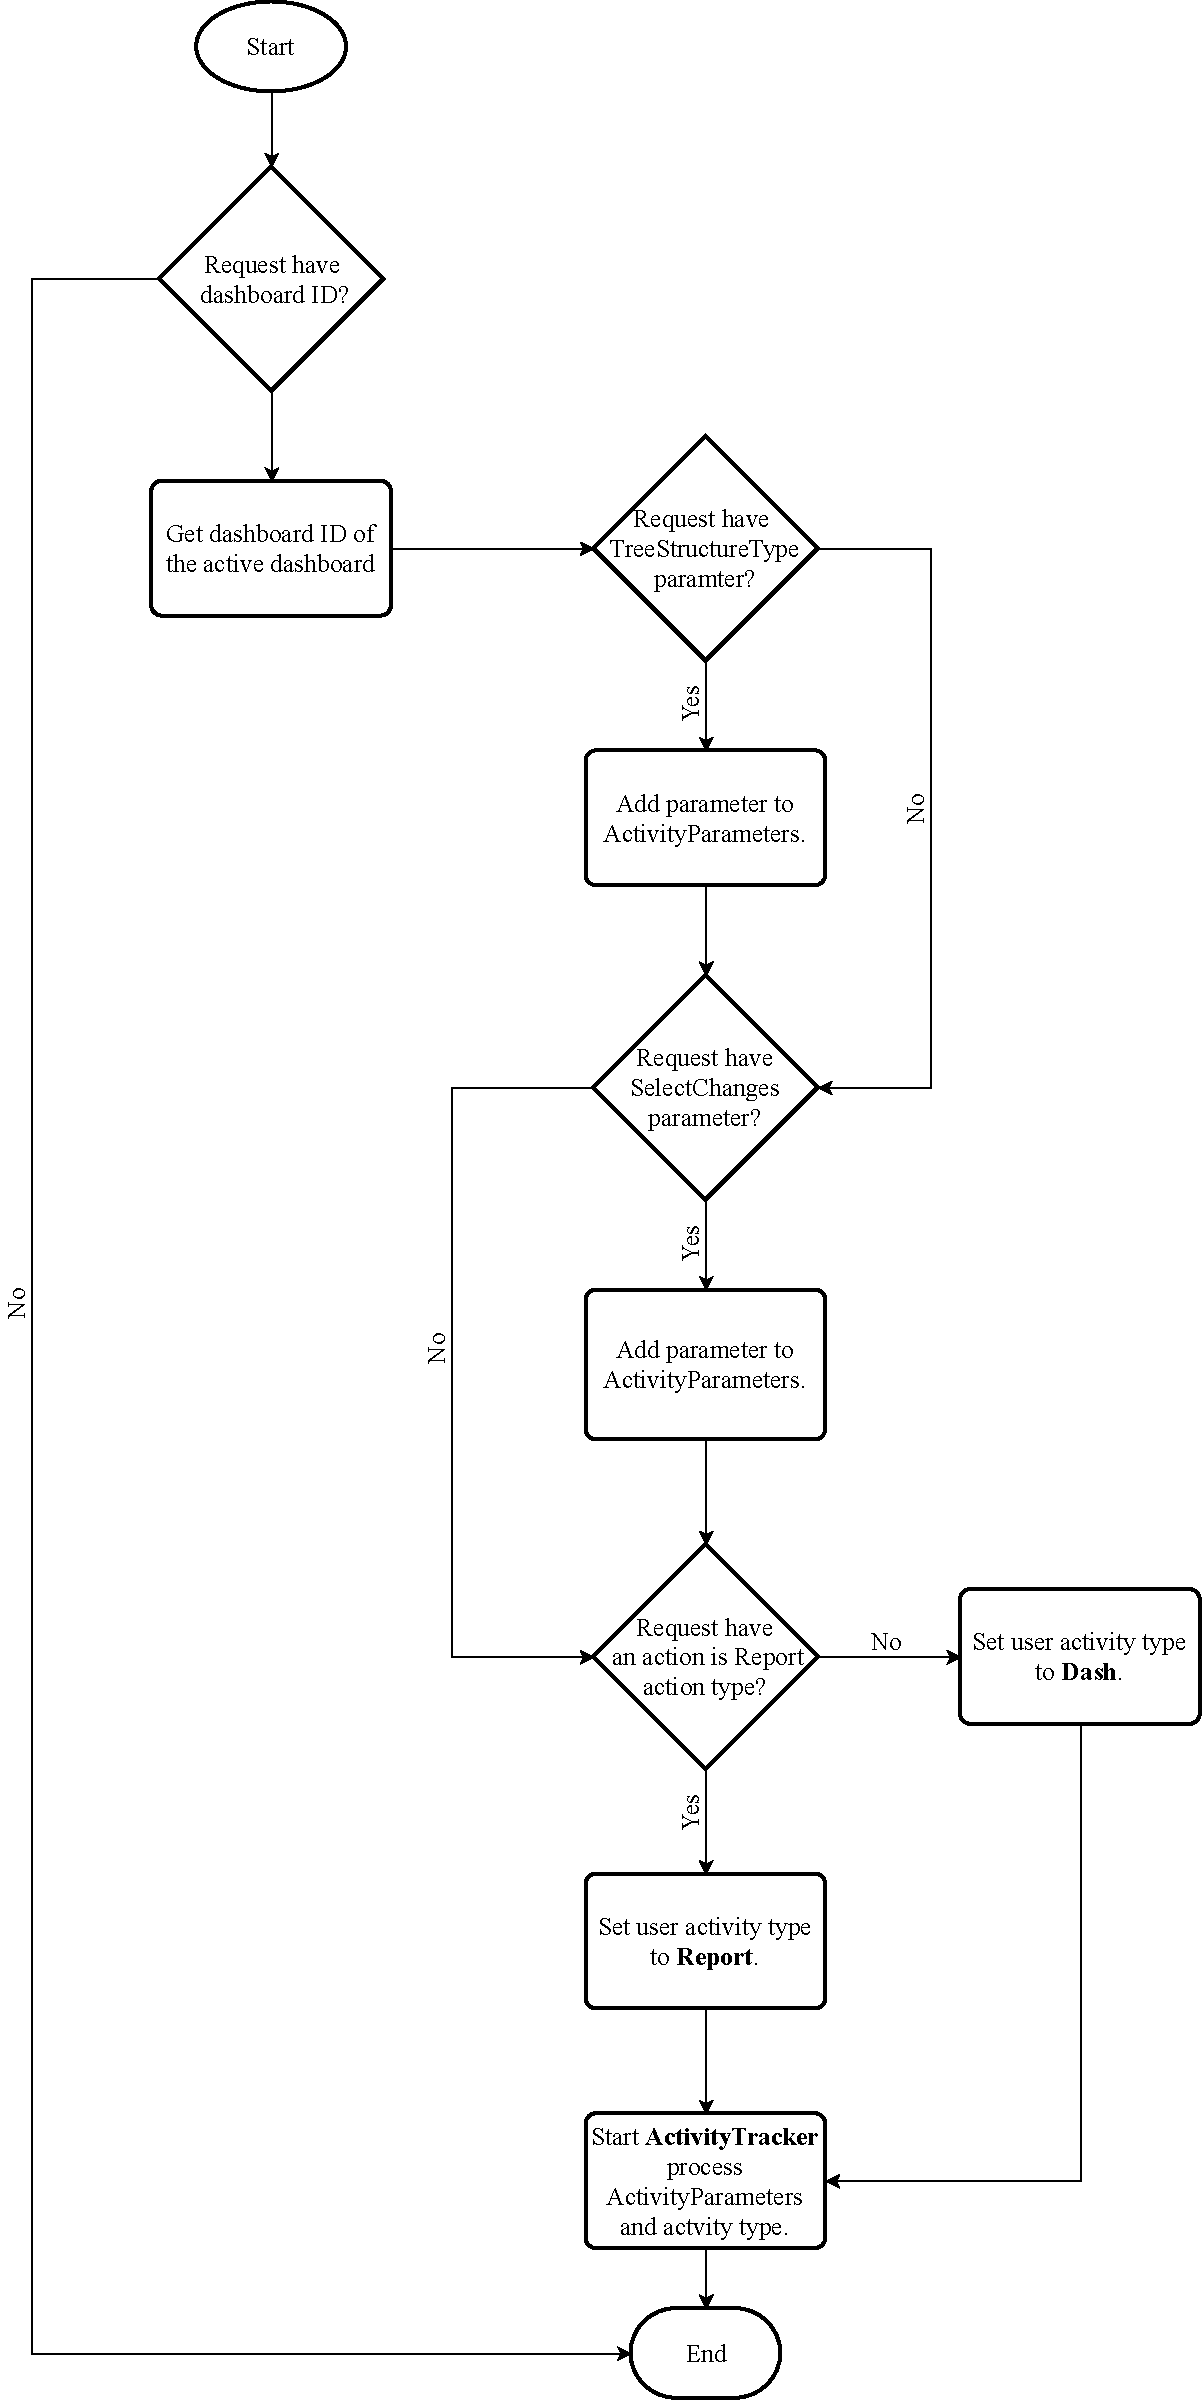
\includegraphics[width=0.7\textwidth]{Chapter2/Dash_PHP_Flow/Dash_PHP_Flow.pdf}
	\caption[User activity logging of Dash and Report event types]
	{\textit{User activity logging process of Dash and Report event types flow diagram}}\label{fig:ch2_Dash_PHP_Flow}
\end{figure}

\clearpage

\subsubsection{User activity logging process of DetailView and Report event types}

In \Cref{fig:ch2_DetailView_Flow} is the process of getting the DetailView and Report user activity event type for System A. This logging process is used in each file that dashboards are created from. In \Cref{fig:ch2_SystemA_Dashboard} multiple dashboards can use the same files with different configuration parameters send with the request, therefore this significantly reduces the needed development to enable the user activity tracking for the dashboards.\par After the user has navigated to their selected dashboard, any user generated request is logged as user activities in System A. These events can be divided into the DetailView and Report event types based on their action parameters that is send with the request. If the event doesn't have any action parameters, the logging process terminates as this event doesn't count as a valid user activity event.\par If the event does have any action parameters it is checked whether the parameters have report generation value or not. If the event have report action values then the user activity type is set to the Report event type otherwise it is set to DetailView event type.\par There may exist any additional parameters that is send with the request that can be logged. These parameters will vary more than the additional parameters of the Dash events as the Dash events parameters is used to configure the dashboard and not get certain variations activities the user performs on the dashboard.\par If the additional parameters are not null or empty values they are added to the ActivityParameters. With the set ActivityParameters and the defined user activity type the ActivityTracker process of \Cref{fig:CH2_SystemA_DB_Interaction_FlowDiagram} to create a log entry that is saved in the SQL database.

\begin{figure}[!htb] % An h :here, t: top, b: bottom.
	\centering % cent the figure
	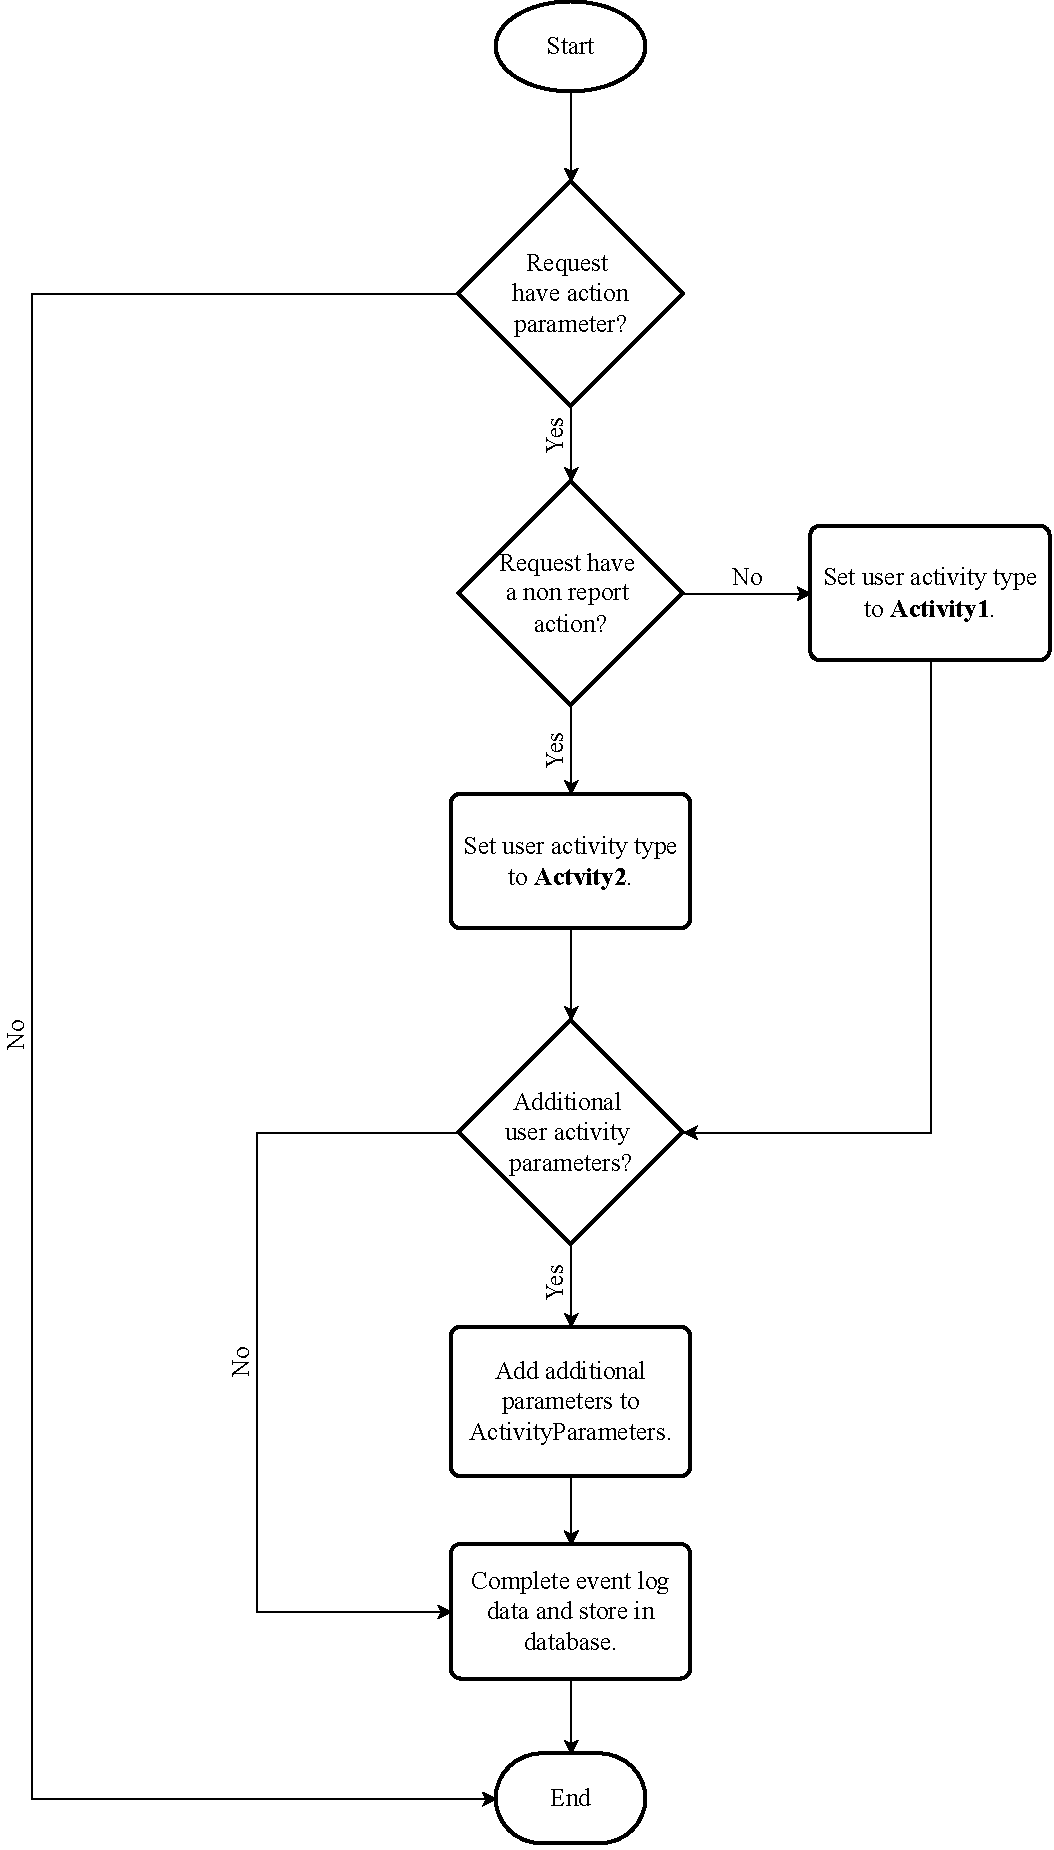
\includegraphics[width=0.75\textwidth]{Chapter2/DetailView_Flow/DetailView_Flow.pdf}
	\caption[User activity logging of DetailView and Report event types]
	{\textit{User activity logging process of DetailView and Report event types flow diagram}}\label{fig:ch2_DetailView_Flow}
\end{figure}

\clearpage

\subsubsection{Database interaction of the logging mechanism}\label{sec:CH2_SystemA_DB_Interaction_FlowDiagram}

In \Cref{fig:ch2_Dash_PHP_Flow,fig:ch2_DetailView_Flow} the user generated event is captured with additional parameters that may exist with the captured event. The next process in \Cref{fig:CH2_SystemA_DB_Interaction_FlowDiagram} is save the generated user activity log in a database.\par \Cref{fig:CH2_SystemA_DB_Interaction_FlowDiagram} is the process which the logging mechanism will create a log entry by first initialising the SQL database connection. The last parameter needed to complete the requirements of the logging points in \Cref{tbl:Ch2_System_A_Logging_Points} is the user's identification. This is obtained from the user's session that contains the user's ID number that is assigned in the Users table.\par The ActivityParameters from  \Cref{fig:ch2_Dash_PHP_Flow,fig:ch2_DetailView_Flow} are encoded as a JSON string to be saved in the RequestParameters column. After all the parameters are converted to correct format the SQL query created and executed to save the log entry in the SystemA\_UserActivities table of \Cref{fig:Ch2_SystemA_Basic_ERD}.

\begin{figure}[!htb] % An h :here, t: top, b: bottom.
	\centering % cent the figure
	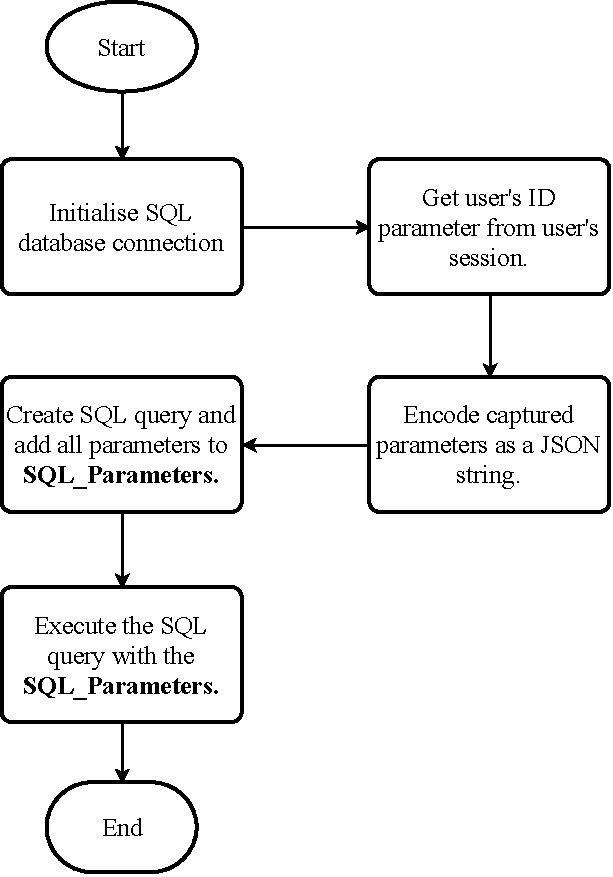
\includegraphics[width=0.5\textwidth]{Chapter2/SystemA_ActivityTracker/SystemA_ActivityTracker.pdf}
	\caption[User activity logging mechanism database interaction]
	{\textit{User activity logging mechanism database interaction}}\label{fig:CH2_SystemA_DB_Interaction_FlowDiagram}
\end{figure}

\clearpage

\subsection{System B}

\subsubsection{System B's logging points}

In \Cref{fig:ch2_Flow_MVC_Architecture} is a diagram of the request flow of a MVC architecture that shows how the user interacts with it. The user will send multiple request from their own device (client device) via an Internet connection to the server that process the request. The software system will read and write data the database source to create a result that send back to the client device for the user. System B is based on this type of architecture to display multiple menus to the user. 

\begin{figure}[!htb] % An h :here, t: top, b: bottom.
	\centering % cent the figure
	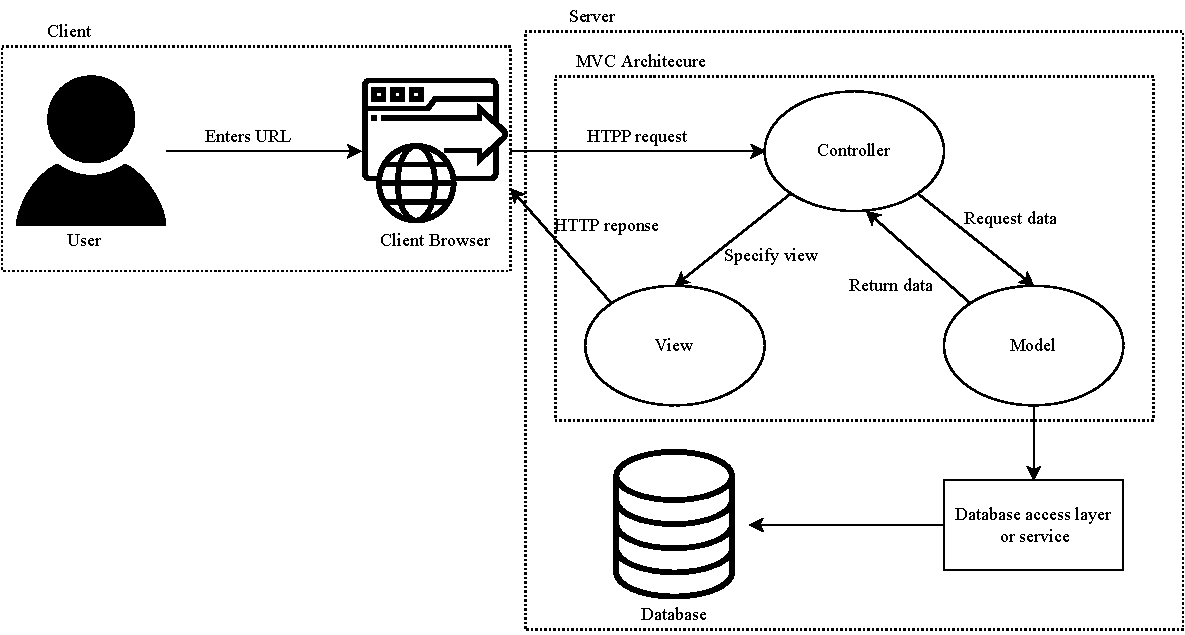
\includegraphics[width=0.95\textwidth]{Chapter2/Flow_MVC_Architecture/Flow_MVC_Architecture.pdf}
	\caption[Request flow in MVC architecture]
	{\textit{Request flow in MVC architecture \cite{Gu2010}}}\label{fig:ch2_Flow_MVC_Architecture}
\end{figure}

In \Cref{sec:SystemA_LoggingPoints} System A mostly relies on the user sessions data to obtain the user generated event's data, for System B this data can be obtained by the FilterContext class in ASP.NET MVC. The FilterContext provides contains the following information about the request:

\begin{itemize}
	\item \textbf{Absolute URI path:} The string containing the absolute URI path the current controller that is active is part of the FilterContext. This does not reference the controller that handles the request but the controller that user is active on before initiating the request. 
	\item \textbf{Absolute request URL:} The request URL contains the controller's name and function that process requests. This reference the controller that handles the request but the controller that user is active on before initiating the request. Most of System B's menus are partitioned in separate units which is called Areas in the ASP.NET MVC projects. The area from which the controller is from is also part of the of this path.
	\item \textbf{Action parameters:} The FilterContext contains action parameters which are the request parameters send with the AJAX request from the client device. These parameters are used in the function that is being called to do certain task within the controller.
\end{itemize}

In System B's session information the user's identification credentials are stored and is used to identify which user initiated the event that is processed.

\clearpage

Using the information from the FilterContext and session of System B the key logging points can be obtained to create \Cref{tbl:CH2_SystemB_LoggingTable} that is saved in SQL database. Each of this logging points can be accessed through a filter action to capture run-time data such as the action parameters that is part of the meta data.

\begin{table}[!htb]
	\centering
	\small
	\caption[System B user activities table]
	{\textit{System B user activities table}}
	\label{tbl:CH2_SystemB_LoggingTable}
	\begin{tabularx}{\textwidth}{|l|l|X|}
		\hline \textbf{Column Name} & \textbf{SQL Data Type} & \textbf{Description} \\
		\hline \textbf{ActivityID} & INT(11) & The activity identification is an incremental number of the event that is logged.\\
		\hline \textbf{Timestamp} & DATETIME & This is the time which the event took place.\\
		\hline \textbf{ActivityType} & ENUM & Each event that the user initiate has an activity type as in \Cref{tbl:Ch2_SystemB_ActivityTypes}. This activity type is dependent if the controller's called method is the index action or based on the HTML element that is part of the meta data. \\
		\hline \textbf{UserID} & INT(4) & Each user has a unique identifier which is a numerical identification number that is foreign key reference to the User table. \\
		\hline \textbf{Area} & VARCHAR(45) & This information is logged to track user activities per Area that represents different software systems that the user can use. \\
		\hline \textbf{Controller} & TEXT & Each event will point back to an controller that process the request. \\
		\hline \textbf{GroupID} & INT(4) & This foreign key reference to the Group table is contract groups identification number. \\
		\hline \textbf{MetaData} & JSON & The meta data of the event contains request parameters, the HTML element from which the request is initiated and other relevant request data of the event. This can also be other meta data is important to get that adds more information about the user's activity using certain controls on System B as in \Cref{fig:CH2_SystemBMetaData}. \\
		\hline
	\end{tabularx}
\end{table}

In \Cref{fig:CH2_SystemBMetaData} the meta data JSON for the user activity log obtained. This JSON contains the request origin of the event from the absolute URI path, HTML element that user used to initiate the event and the request parameters send with the AJAX request. Some of these JSON parameters can be empty depending on the type of the activity.

\begin{figure}[!htb]
	\centering
	\begin{lstlisting}[style=json] 
	{
		"RequestOrigin" : "/Area4/Controller4",
		"RequestElementID" : "Button4",
		"RequestParameters": {
			"Parameter1": 4,
			"Parameter2": "Hello World!",
			"Parameter3": true
			"Parameter4": 40.404
		}
	}
	\end{lstlisting}
	\caption[System B meta data JSON]
	{\textit{System B meta data JSON}}\label{fig:CH2_SystemBMetaData}
\end{figure}

\clearpage

The user activity types in \Cref{tbl:Ch2_SystemB_ActivityTypes} is all of the possible activities the user can generate in System B. The MenuAccessed activity type can be used to track how the user is navigating through the System B just like System A's Dash user activity type. The CustomControls and ElementClickEvents user activity types is the best representation of the system utilisation of System B by the users.

\begin{table}[!htb]
	\centering
	\small
	\caption[System B user activity types]
	{System B user activity types}
	\label{tbl:Ch2_SystemB_ActivityTypes}
	\begin{tabularx}{\textwidth}{|l|X|}
		\hline \textbf{Activity Type} & \textbf{Description} \\
		\hline \textbf{MenuAccessed} & These events are any user activities where the user attempts to access a menu on System B which calls the index method of the menu's controller. In most cases the event request from the client side will be handled by the controller's index function to send back a response of the initial accessing of a specific menu. \\
		\hline \textbf{LogoutAttempt} & Any logout attempt from the user except closing the browser tab or browser. Closing the browser or tab doesn't send any request from the client device back to the server to log that user ended their session. \\
		\hline \textbf{LoginAttempt} & Any user activities on the login page of System B where the user will try enter their credentials to gain access to their user accounts on System B.\\
		\hline \textbf{SessionTracking} & This is any user activities that directly involves extension session due that System B will attempt to logout the user after a hour of inactivity prompting the user to extend their own session.\\
		\hline \textbf{ResetPassword} & Any user activities when the user attempts to reset their password. \\
		\hline \textbf{CustomControls} & System B uses custom controls made the development team, when the user uses these controls it will also initiated an event that can be tracked. \\ 
		\hline \textbf{ElementClickEvents} & Any distinguishable \emph{HTML} element that is clicked by the user that communicates back to the server. These events are ButtonClicked, SelectClicked, ImageClicked, InputClicked, SpanClicked, LabelClicked, ListClicked, HyperLinkClicked, DivClicked, FormInput and GridItem.\\
		\hline
	\end{tabularx}
\end{table}

In \Cref{fig:ch2_SystemB_Basic_ERD} is the ERD of tables directly used for System B. The key logging points of \Cref{tbl:CH2_SystemB_LoggingTable} is used to create the table SystemB\_UserActivities. The data is stored in a SQL database where the Users and Groups tables are. The Users table contains all the information of the users using the System B and the Groups table contains all the mine contract group information. 

\begin{figure}[!htb] % An h :here, t: top, b: bottom.
	\centering % cent the figure
	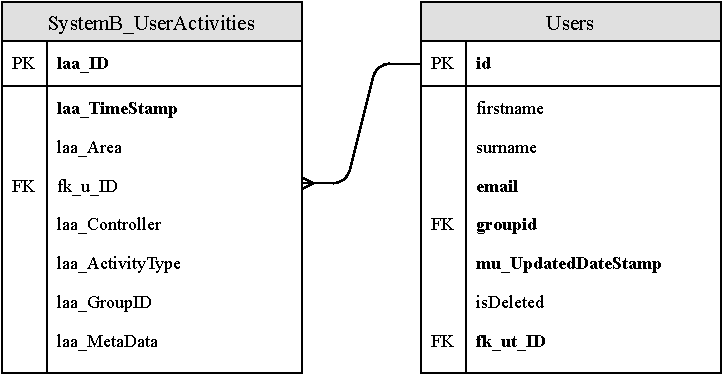
\includegraphics[width=0.99\textwidth]{Chapter2/SystemB_ERD_Basic/SystemB_ERD_Basic.pdf}
	\caption[System B user activity ERD]
	{\textit{System B user activity ERD}}\label{fig:ch2_SystemB_Basic_ERD}
\end{figure}

\clearpage

\begin{figure}[!htb]
	\centering
	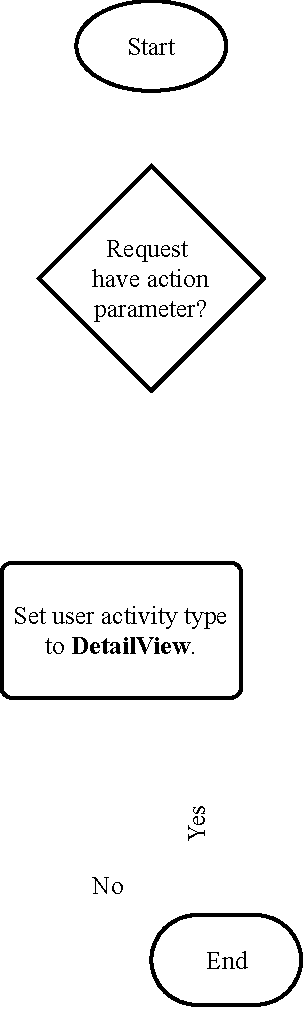
\includegraphics[width=0.2\textwidth]{Chapter2/SystemB_Javascript_EventTracker/SystemB_Javascript_EventTracker.pdf}
	\caption[System B user generated event capture]
	{\textit{System B user generated event capture flow diagram}}\label{fig:CH2_SystemB_EventCapture}
\end{figure}

\clearpage

\begin{figure}[!htb]
	\centering
	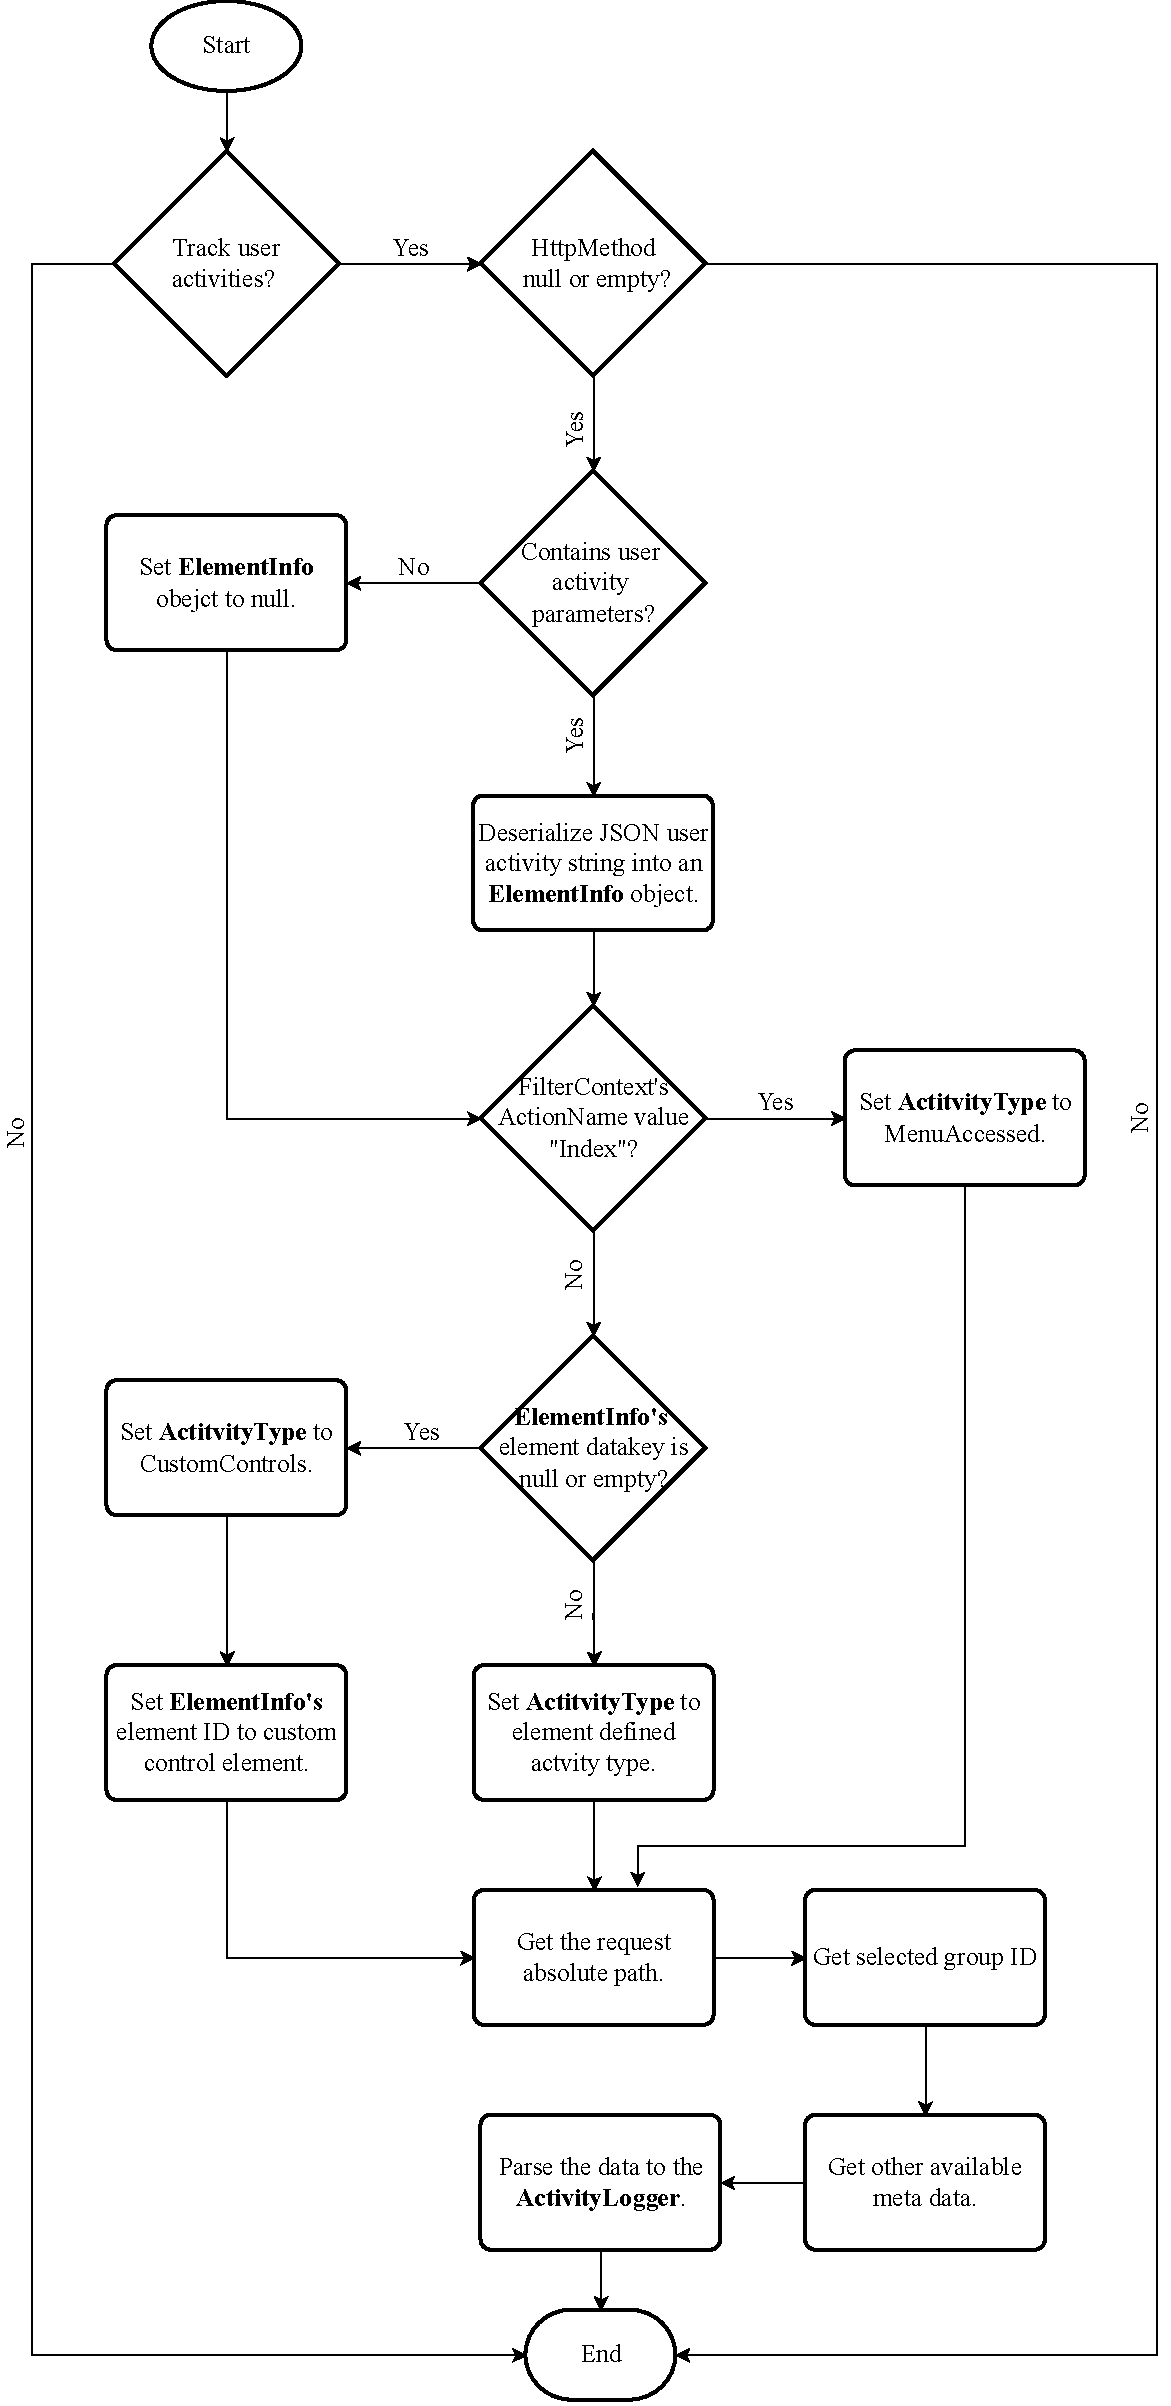
\includegraphics[width=0.7\textwidth]{Chapter2/SystemB_FilterContext/SystemB_FilterContext.pdf}
	\caption[System B event classification]
	{\textit{System B event classification flow diagram}}\label{fig:CH2_SystemB_FilterContext}
\end{figure}

\clearpage

\section{System utilisation analysis}

\section{Integration}
In this section the integration of the utilisation analysis and logging mechanism will be discussed.

\section{Conclusion}
Conclude the chapter about the development of the logging mechanism and utilisation analysis.